%%%%%%%%%%%%%%%%%%%%%%%%%%%%%%%%%%%%%%%%%%%%%%%%%%%%%%%%%%%%%%%%%%%%%%%%%%%%%%%
\chapter{Experimental setup and results}~\label{chap:results}
%%%%%%%%%%%%%%%%%%%%%%%%%%%%%%%%%%%%%%%%%%%%%%%%%%%%%%%%%%%%%%%%%%%%%%%%%%%%%%%

A Linux kernel module was developed incorporating the ideas mentioned in chapters \ref{chap:pds}
and \ref{chap:delta}. The scheduling routines in the Linux kernel (To be specific, \textit{schedule} and \textit{\_\_switch\_to})
were extended using kprobes \cite{kprobes} to add the performance directed scheduling features
The entire system with all the interconnections is shown in figure \ref{fig:entire_seeker}.

The choice to use kprobes \cite{kprobes} a feature essentially used for debugging and instrumentation
from the context of a kernel module pose two possible 
problems. One, kprobes by themselves introduce unnecessary code paths and interrupts causing some
if not significant overhead (Less than 3\% overhead). Secondly, certain functions relating to migration are not exported
to kernel modules and hence indirect and suboptimal procedures were chosen to get the necessary 
functionality. In spite of these disadvantages, having the project as a kernel module accelerated 
the development process. 

For a system with \textit{M} total performance states and \textit{N} total processors, $\Delta$ can 
at most take a value of $N \times (M-1)$. Experiments were carried on a quad-core AMD Opteron (Barcelona),
with mutation intervals ranging from 125ms to 1000ms and delta ranging from 1 through 16. The experiments
were carried out with full logging enabled and all of the six different workloads described in Appendix~\ref{app:benchmark}. 
The logs taken contained information relating to the residency of each processor in each state and was 
translated to average power consumed per processor by correlating it to the numbers mentioned in \cite{AMDPow} and
repeated in Appendix~\ref{app:opteron}. 


\begin{figure}[h!]
  \begin{center}
%    \resizebox{\columnwidth}{!}{
    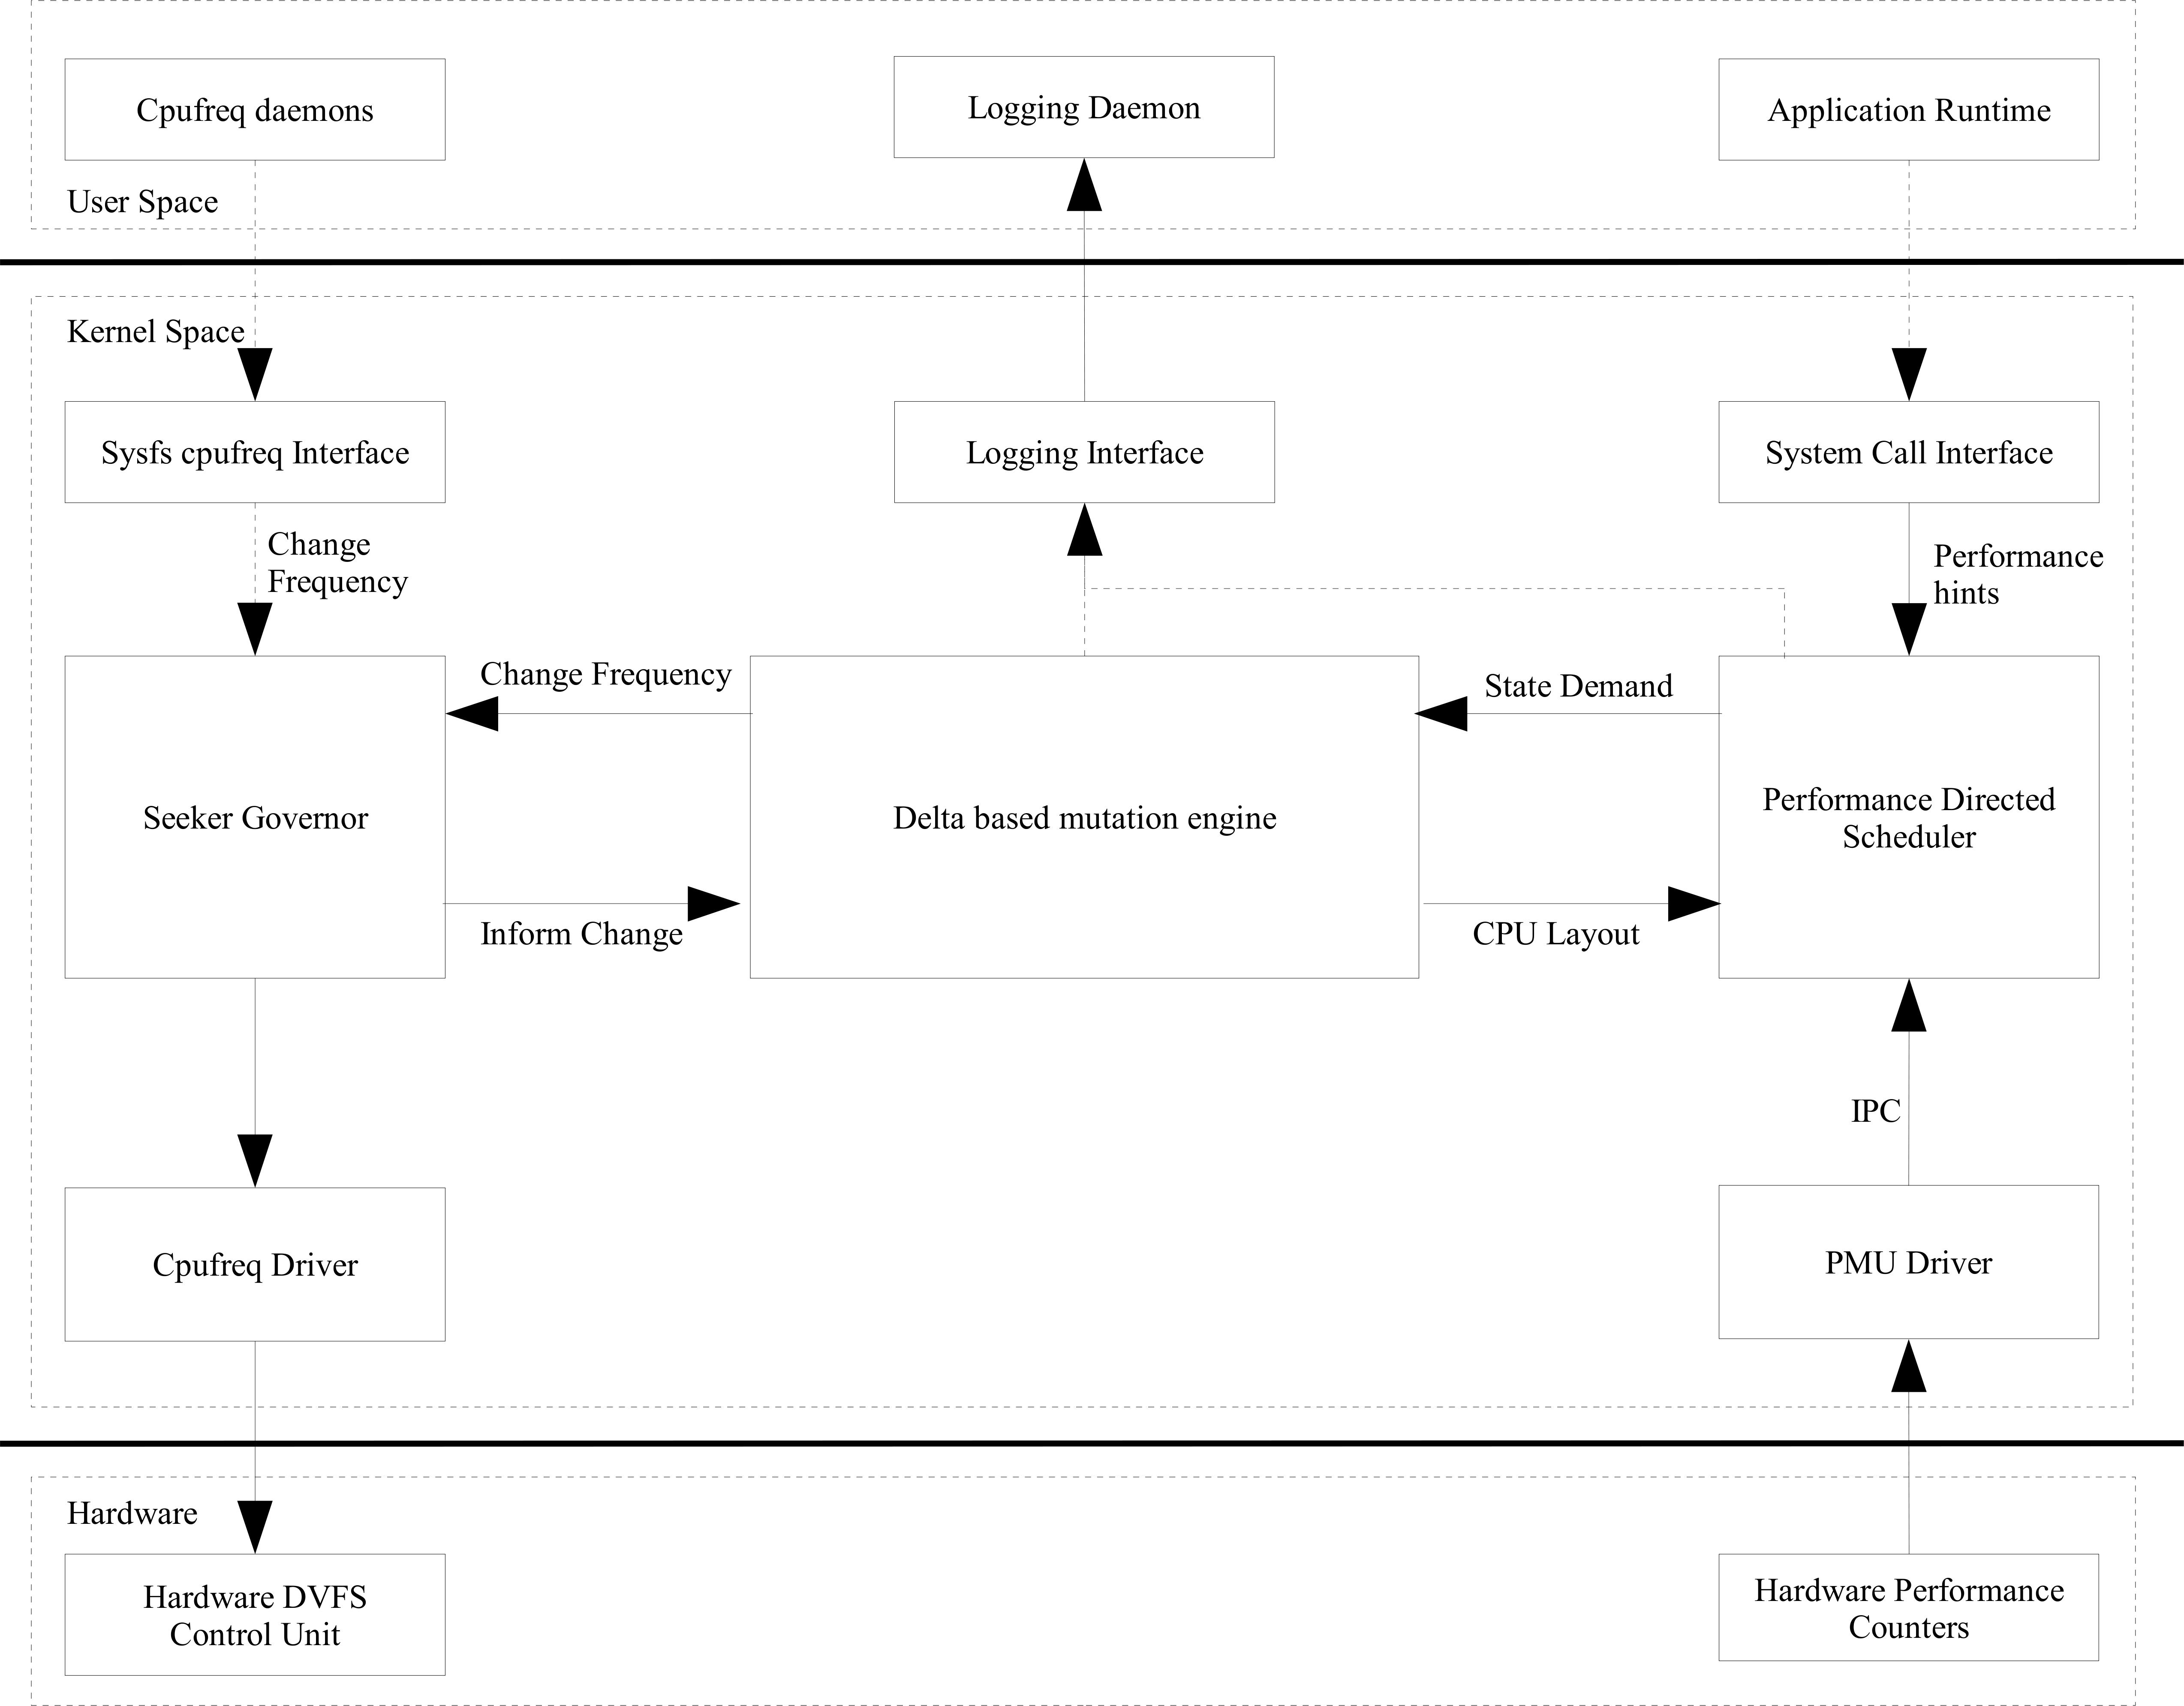
\includegraphics[height=4in]{figures/seeker.jpg}%}
    \caption{The Seeker infrastructure}
    \label{fig:entire_seeker}
  \end{center}
\end{figure}


Three different configurations were run on repeated trials: 
\begin{enumerate}
\item Ondemand governor with scheduling disabled. 
\item Delta mutation engine with the ladder scheduler
\item Delta mutation engine with the select scheduler
\end{enumerate}
The results following which are discussed in further sections. 

%%%%%%%%%%%%%%%%%%%%%%%%%%%%%%%%%%%%%%%%%%%%%%%%%%%%%%%%%%%%%%%%%%%%%%
% START REAL GRAPHS
%%%%%%%%%%%%%%%%%%%%%%%%%%%%%%%%%%%%%%%%%%%%%%%%%%%%%%%%%%%%%%%%%%%%%%
%%%%%%%%%%%%%%%%%%%%%%%%%%%%%%%%%%%%%%%%%%%%%%%%%%%%%%%%%%%%%%%%%%%%%%%%%%%%%%%
\section{Trends along delta and interval}~\label{sec:trends}
%%%%%%%%%%%%%%%%%%%%%%%%%%%%%%%%%%%%%%%%%%%%%%%%%%%%%%%%%%%%%%%%%%%%%%%%%%%%%%%

Figures \ref{fig:slowdown_trends_ladder} and \ref{fig:slowdown_trends_select} show the trends
observed with respect to slowdown for the ladder and select schedulers. An unnaturally 
high slowdown can be observed for small values of delta ($\Delta$). This can easily be attributed
to the plasticity in adaptation. The interval of mutation has little significance towards slowdown
towards delta values beyond 3. But it is observed to play a vital role at lower values of delta 
where an increase in the mutation interval causes an adverse increase in the slowdown thus 
agreeing with the hypothesis of plastic adaptation. Figures \ref{fig:pwr_trends_ladder} and
\ref{fig:pwr_trends_select} which are the average power savings studied with varying degrees
of delta and mutation interval are similar to that of slowdown. 

\begin{figure}[h!]
  \begin{center}
    %\resizebox{\columnwidth}{!}{
    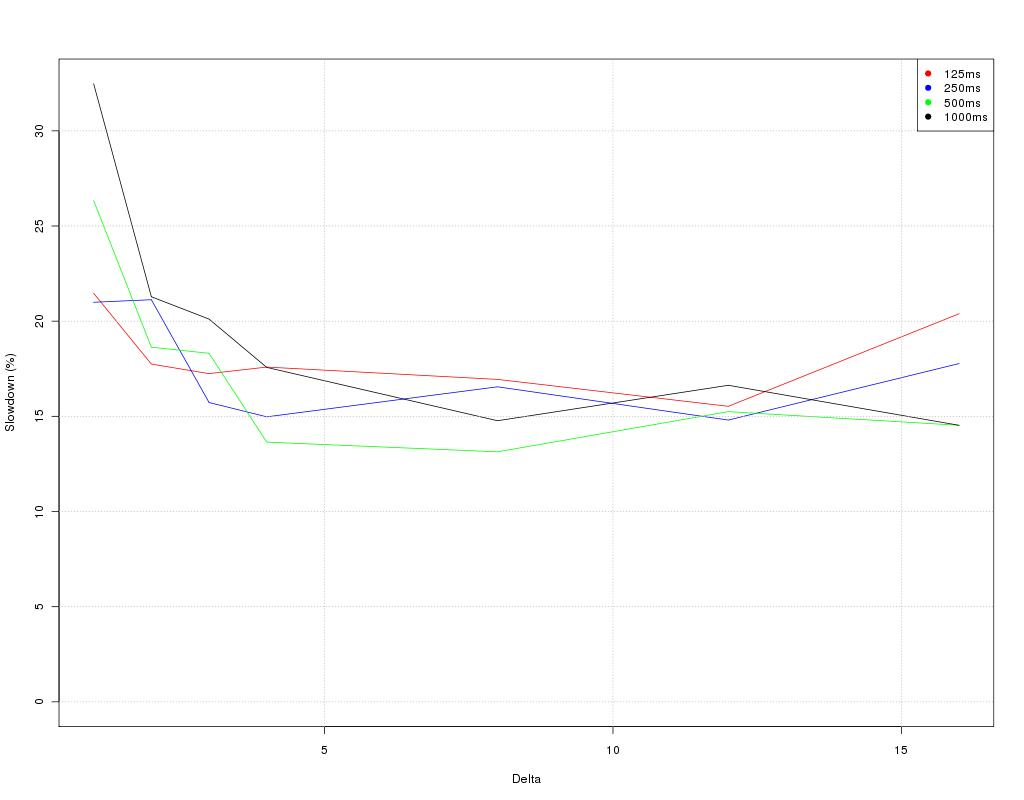
\includegraphics[height=3.5in]{figures/trends_slowdown_ladder.jpg}%}
    \caption{Variation of slowdown with delta and interval with the ladder scheduler}
    \label{fig:slowdown_trends_ladder}
  \end{center}
\end{figure}

\begin{figure}[h!]
  \begin{center}
    %\resizebox{\columnwidth}{!}{
    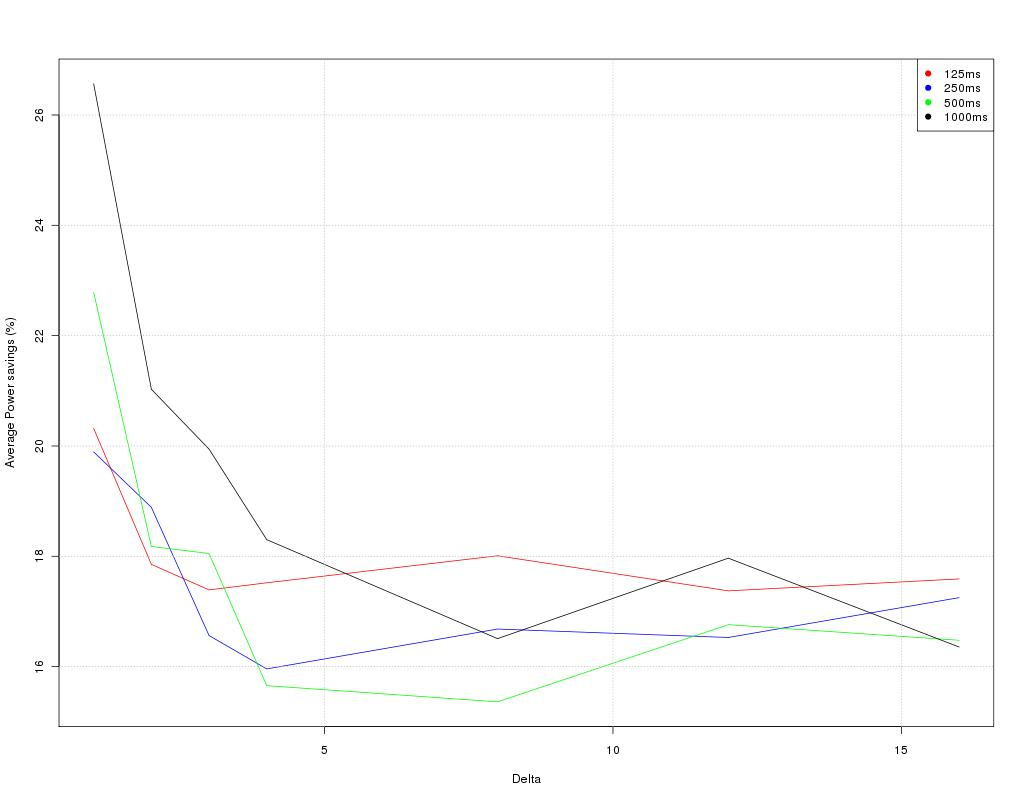
\includegraphics[height=3.5in]{figures/trends_avgpwr_ladder.jpg}%}
    \caption{Variation of power savings with delta and interval with the ladder scheduler}
    \label{fig:pwr_trends_ladder}
  \end{center}
\end{figure}

% NEEDS TO BE RE-GENERATED.
\begin{figure}[h!]
  \begin{center}
    %\resizebox{\columnwidth}{!}{
    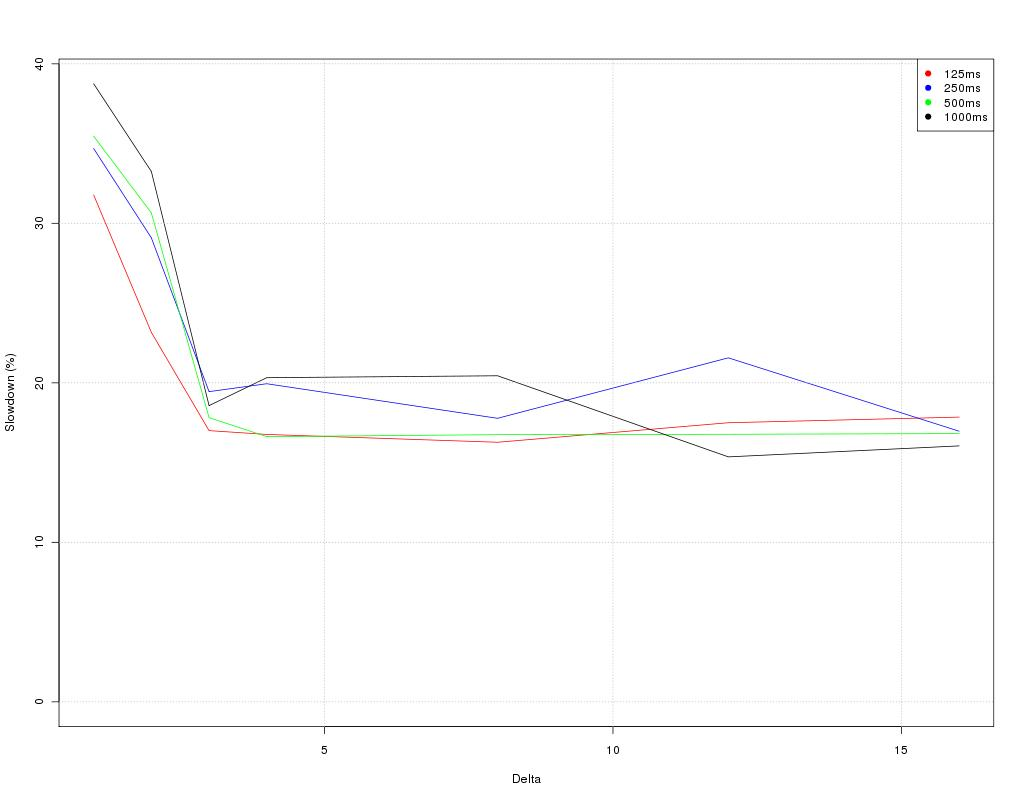
\includegraphics[height=3.5in]{figures/trends_slowdown_select.jpg}%}
    \caption{Variation of slowdown with delta and interval with the select scheduler}
    \label{fig:slowdown_trends_select}
  \end{center}
\end{figure}

% NEEDS TO BE RE-GENERATED.
\begin{figure}[h!]
  \begin{center}
    %\resizebox{\columnwidth}{!}{
    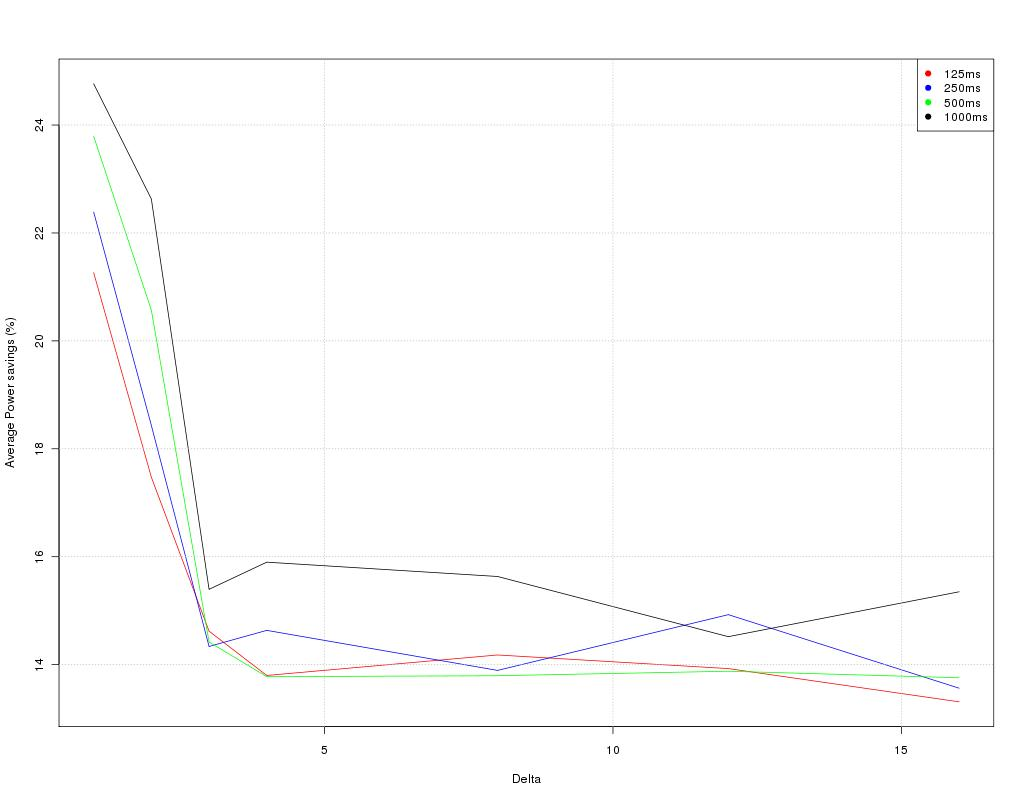
\includegraphics[height=3.5in]{figures/trends_avgpwr_select.jpg}%}
    \caption{Variation of power savings with delta and interval with the select scheduler}
    \label{fig:pwr_trends_select}
  \end{center}
\end{figure}

Due to the adaptive nature of the power management mechanism, it can be hypothesized
that workloads with lower IPC (The \textit{Low} workload) should expect the maximum
power savings while, workloads with a large IPC (The \textit{High} workload) should
expect the minimum slowdown and power savings. This is validated from Figures \ref{fig:workload_trends_ladder}
and \ref{fig:workload_trends_select}. As slowdown is expected, the advantage of the procedure
is the higher power savings than slowdown which both the select and ladder scheduling
procedures exhibit. 

\begin{figure}[h!]
  \begin{center}
    %\resizebox{\columnwidth}{!}{
    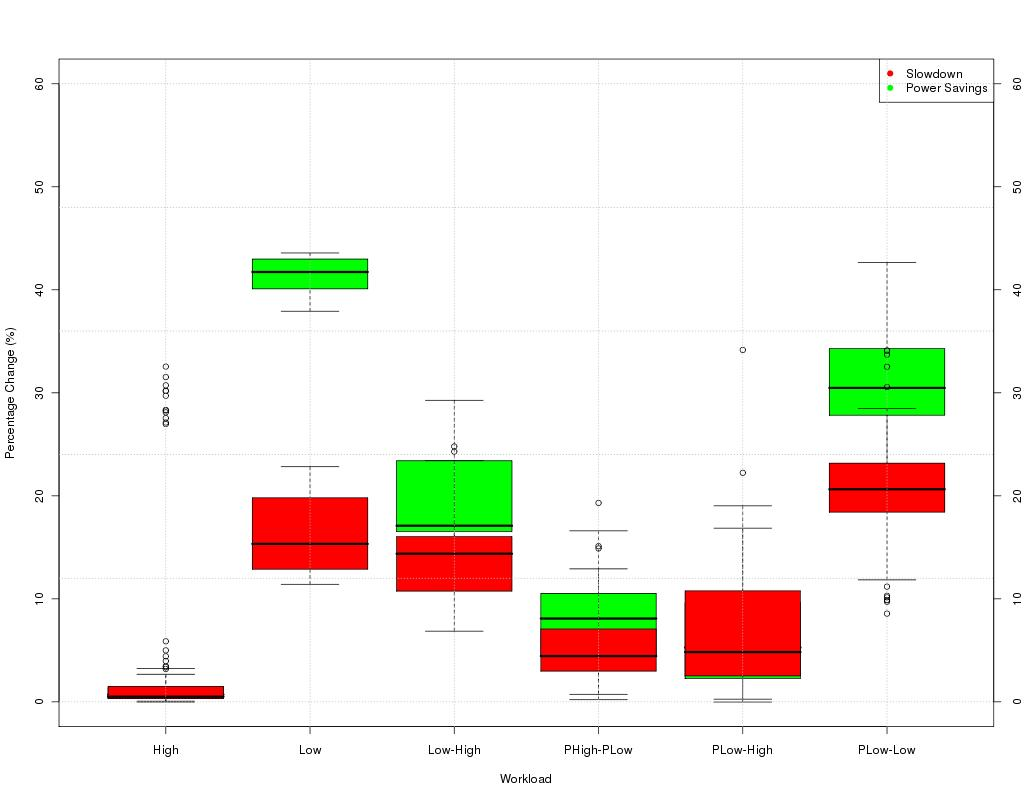
\includegraphics[height=3.5in]{figures/trends_workload_ladder.jpg}%}
    \caption{Variation of slowdown and power savings for each workload with the ladder scheduler}
    \label{fig:workload_trends_ladder}
  \end{center}
\end{figure}

% NEEDS TO BE RE-GENERATED.
\begin{figure}[h!]
  \begin{center}
    %\resizebox{\columnwidth}{!}{
    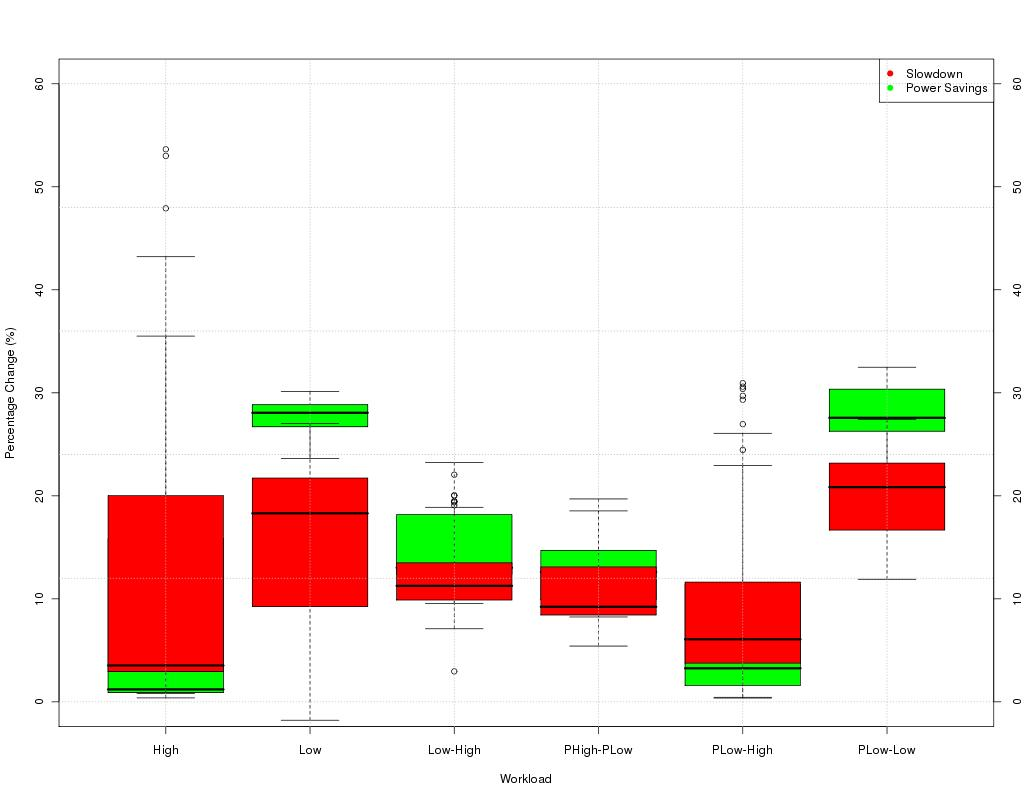
\includegraphics[height=3.5in]{figures/trends_workload_select.jpg}%}
    \caption{Variation of slowdown and power savings for each workload with the select scheduler}
    \label{fig:workload_trends_select}
  \end{center}
\end{figure}

%%%%%%%%%%%%%%%%%%%%%%%%%%%%%%%%%%%%%%%%%%%%%%%%%%%%%%%%%%%%%%%%%%%%%%%%%%%%%%%
\section{Comparing various methodologies}~\label{sec:compare}
%%%%%%%%%%%%%%%%%%%%%%%%%%%%%%%%%%%%%%%%%%%%%%%%%%%%%%%%%%%%%%%%%%%%%%%%%%%%%%%

In order to provide a more detailed comparison between the various methodologies
(Ondemand, Delta + Select, Delta + Ladder), they need to be equated. As the \textit{Ondemand}
governor does not have a concept of delta, comparisons were made by observing 
the values of the delta mutation for $\Delta = 4$. Scatter plots were drawn to 
observe the raw data as they are more descriptive of outliers and easier to judge.

Figure~\ref{fig:pwr_vs_slowdown} shows a scatter plot of slowdown plotted against power savings. Points
lower indicate a smaller magnitude of slowdown while points farther to the right indicate better power
savings. This graph clearly shows the vice of the Ondemand governor: It does not manage power at active
load and obvious from it's design considerations. This is graphically depicted by all the points pertaining
to the ondemand governor huddled around Power Savings = 0\% and hence providing absolutely no power savings
while the processors are actively executing jobs. The Delta + Select system provides an equal power savings
as the Delta + Ladder except for the workload \textit{Low} for which the ladder system works better in achieving
higher power savings.

% NEEDS TO BE RE-GENERATED.
\begin{figure}[h!]
  \begin{center}
    %\resizebox{\columnwidth}{!}{
    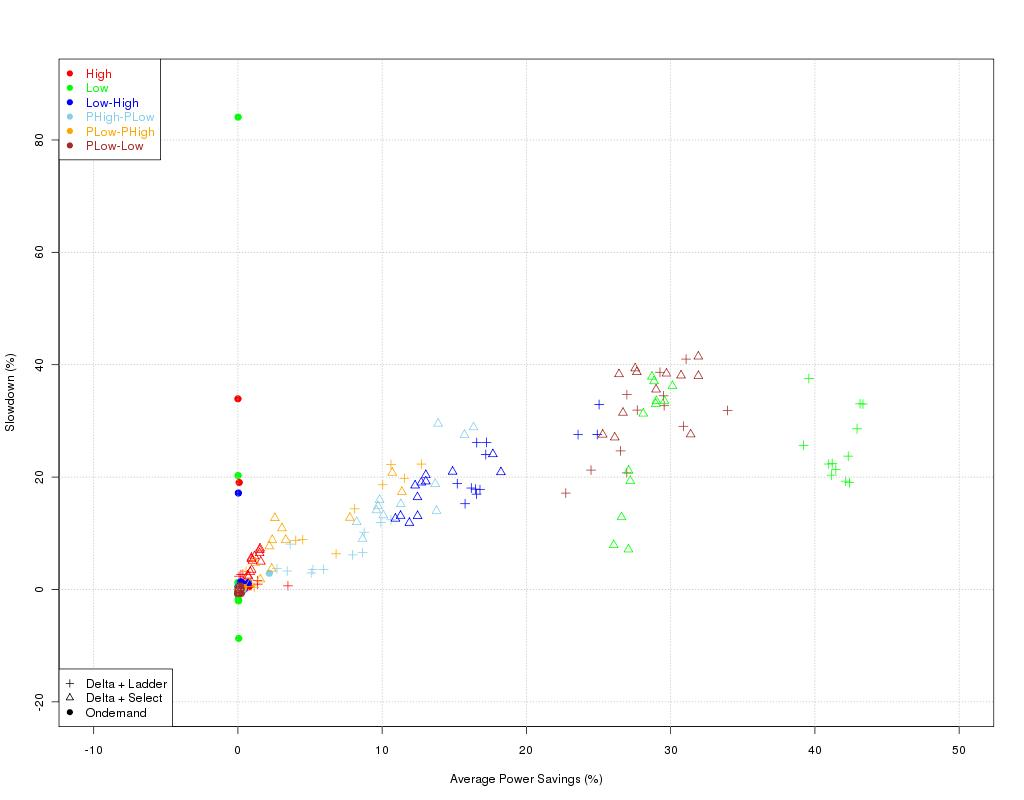
\includegraphics[height=3.5in]{figures/pwr_vs_slowdown_delta_4.jpg}%}
    \caption{Scatter plots showing variation of slowdown with power savings for ondemand, $\Delta=4$ (Select and Ladder)}
    \label{fig:pwr_vs_slowdown}
  \end{center}
\end{figure}

EPI (Energy consumption per instruction) is another important metric which ties in bother throughput and power
consumption. A lower value indicates better energy efficiency. EPI is plotted 
against power savings for each experiment to arrive at Figure~\ref{fig:pwr_vs_jpbi}. As the ondemand governor
does not manage power at execution time, it is observed that not only does it not provide any power savings, 
it ends up utilizing energy inefficiently. 

% NEEDS TO BE RE-GENERATED.
\begin{figure}[h!]
  \begin{center}
    %\resizebox{\columnwidth}{!}{
    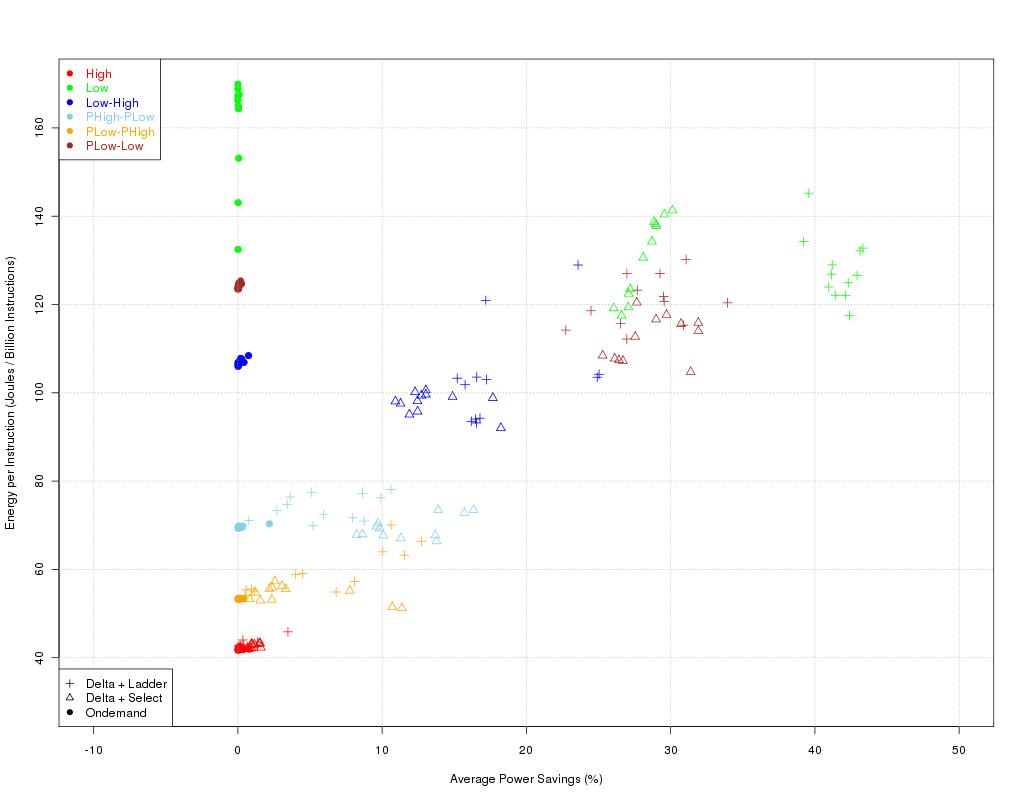
\includegraphics[height=3.5in]{figures/pwr_vs_jpbi_delta_4.jpg}%}
    \caption{Scatter plots showing variation of EPI with power savings for ondemand, $\Delta=4$ (Select and Ladder)}
    \label{fig:pwr_vs_jpbi}
  \end{center}
\end{figure}


An interesting graph \ref{fig:jpbi_vs_slowdown} is arrived at when the scatter plots concentrate on
EPI and slowdown. As we have concluded with figures \ref{fig:pwr_vs_slowdown} and \ref{fig:pwr_vs_jpbi},
the ondemand governor essentially executes all workloads at the highest clock speed (Indicated by 0 slowdown 
and power savings). This allows \ref{fig:jpbi_vs_slowdown} to be viewed to discern if the delta system
does provide a better means to execute workloads in a more energy efficient manner. This is observable
where all the points pertaining to the delta + select and delta + ladder systems lie to the left of 
the ondemand points (Higher as slowdown is expected). 

% NEEDS TO BE RE-GENERATED.
\begin{figure}[h!]
  \begin{center}
    %\resizebox{\columnwidth}{!}{
    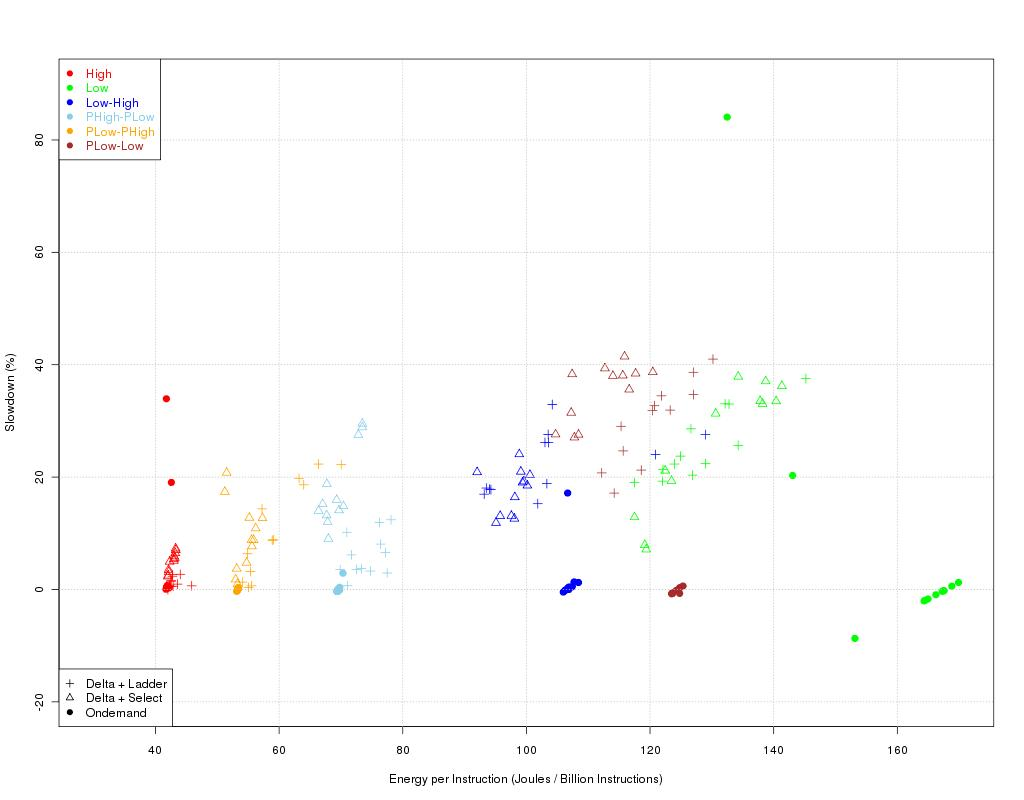
\includegraphics[height=3.5in]{figures/jpbi_vs_slowdown_delta_4.jpg}%}
    \caption{Scatter plots showing variation of slowdown with EPI for ondemand, $\Delta=4$ (Select and Ladder)}
    \label{fig:jpbi_vs_slowdown}
  \end{center}
\end{figure}

%%%%%%%%%%%%%%%%%%%%%%%%%%%%%%%%%%%%%%%%%%%%%%%%%%%%%%%%%%%%%%%%%%%%%%%%%%%%%%%
\section{Power savings and slowdown}~\label{sec:pow_slow}
%%%%%%%%%%%%%%%%%%%%%%%%%%%%%%%%%%%%%%%%%%%%%%%%%%%%%%%%%%%%%%%%%%%%%%%%%%%%%%%

An acceptable power management system demands the relation between power savings and slowdown to be linear
(A slope of 1 at best). Figure~\ref{fig:slowdown_power_ladder} shows a very pleasing slope of 0.9 indicating 
9\% power savings for every 10\% slowdown. 
% rewrite after plotting the remaining run for select. 
But even though the select scheduler is better by hypothesis, it ends up giving closer to 6\% power savings
for every 10\% slowdown (Figure~\ref{fig:slowdown_power_select}). This is probably due to a wrong choice of thresholds. 


\begin{figure}[h!]
  \begin{center}
    %\resizebox{\columnwidth}{!}{
    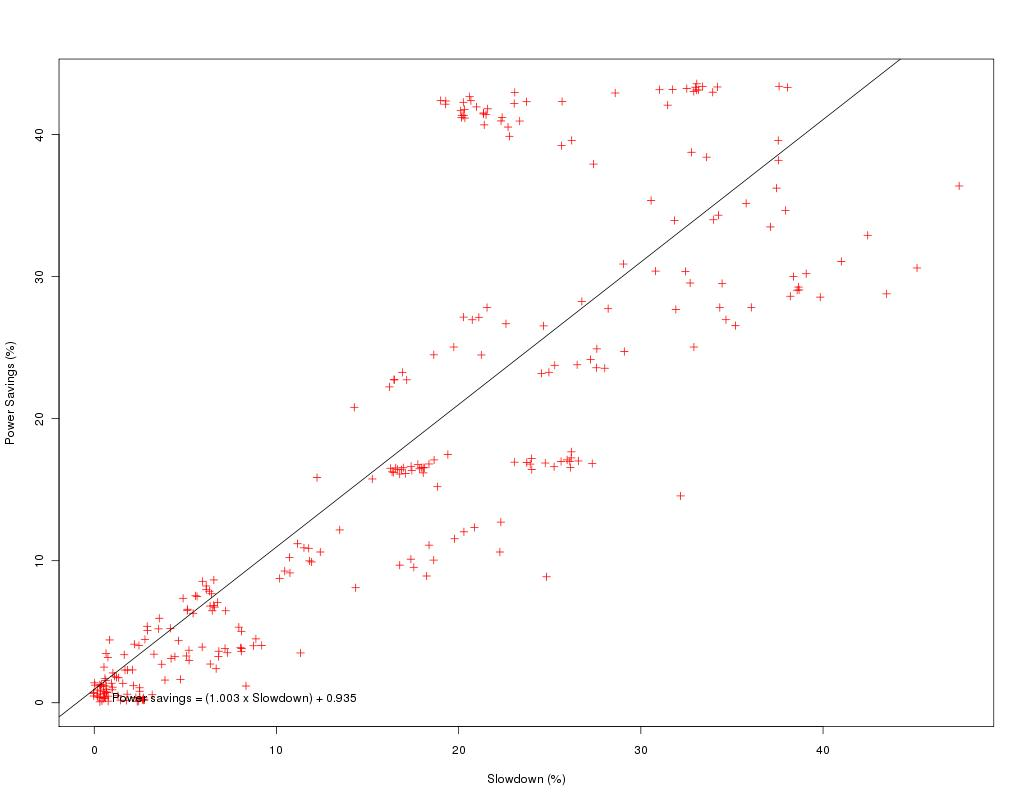
\includegraphics[height=3.5in]{figures/slowdown_power_ladder.jpg}%}
    \caption{Trends over workload variation}
    \label{fig:slowdown_power_ladder}
  \end{center}
\end{figure}

% NEEDS TO BE RE-GENERATED.
\begin{figure}[h!]
  \begin{center}
    %\resizebox{\columnwidth}{!}{
    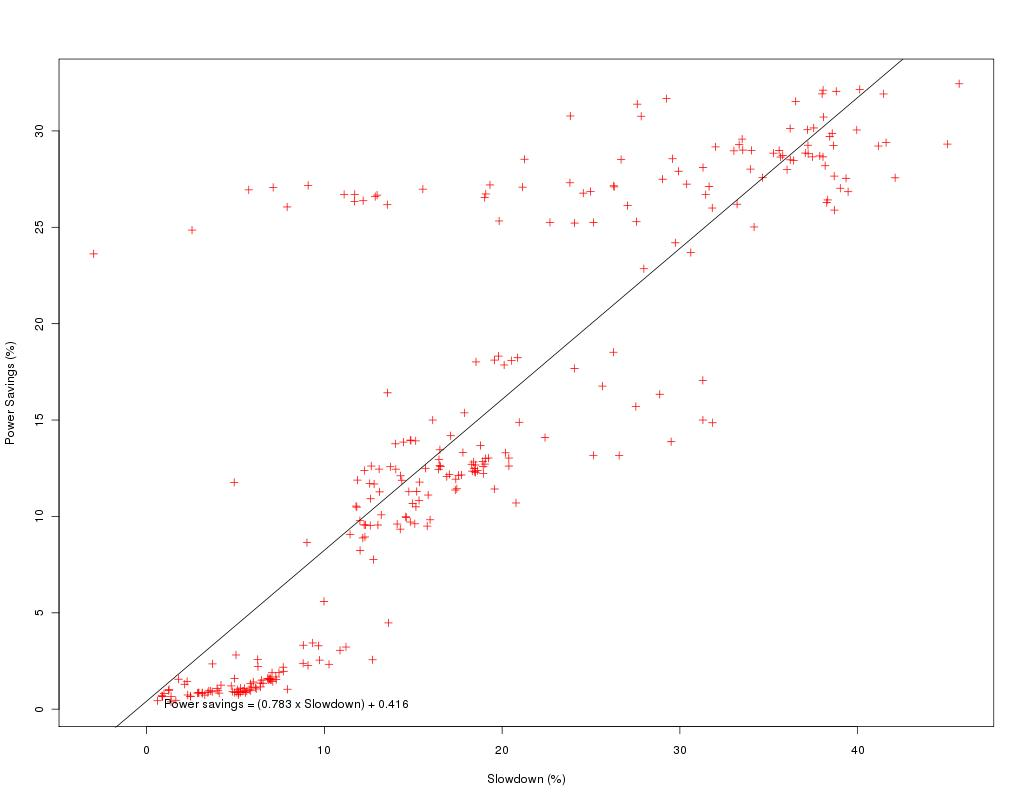
\includegraphics[height=3.5in]{figures/slowdown_power_select.jpg}%}
    \caption{Trends over workload variation}
    \label{fig:slowdown_power_select}
  \end{center}
\end{figure}

%%%%%%%%%%%%%%%%%%%%%%%%%%%%%%
% Do I need to write more? 
%%%%%%%%%%%%%%%%%%%%%%%%%%%%%%
